\chapter*{}
%\thispagestyle{empty}
%\cleardoublepage

%\thispagestyle{empty}

\begin{titlepage}
 
 
\setlength{\centeroffset}{-0.5\oddsidemargin}
\addtolength{\centeroffset}{0.5\evensidemargin}
\thispagestyle{empty}

\noindent\hspace*{\centeroffset}\begin{minipage}{\textwidth}

\centering
%
\includegraphics[width=0.9\textwidth]{imagenes/logo_ugr.jpg}\\[1.4cm]

%\textsc{ \Large PROYECTO FIN DE CARRERA\\[0.2cm]}
%\textsc{ INGENIERÍA EN INFORMÁTICA}\\[1cm]
% Upper part of the page
% 

 \vspace{3.3cm}

%si el proyecto tiene logo poner aquí
%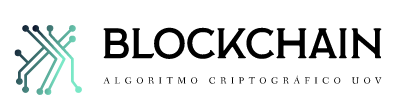
\includegraphics{portada/imagenes/logo.png} 
% \vspace{0.5cm}

% Title

{\Huge\bfseries Implementación de una blockchain resistente a ataques criptográficos post-cuánticos\\
}
\noindent\rule[-1ex]{\textwidth}{3pt}\\[3.5ex]
{\large\bfseries Subtítulo del proyecto.\\[4cm]}
\end{minipage}

\vspace{2.5cm}
\noindent\hspace*{\centeroffset}\begin{minipage}{\textwidth}
\centering

\textbf{Autor}\\ {María Victoria Granados Pozo}\\[2.5ex]
\textbf{Director}\\
{Gabriel Maciá Fernández\\
Francisco Javier Lobillo Borrero 
}\\[2cm]
%
\includegraphics[width=0.15\textwidth]{imagenes/tstc.png}\\[0.1cm]
%\textsc{Departamento de Teoría de la Señal, Telemática y Comunicaciones}\\
%\textsc{---}\\
%Granada, mes de 201
\end{minipage}
%\addtolength{\textwidth}{\centeroffset}
\vspace{\stretch{2}}

 
\end{titlepage}






\cleardoublepage
\thispagestyle{empty}

\begin{center}
{\large\bfseries Implementación de una blockchain resistente a ataques criptográficos cuánticos}\\
\end{center}
\begin{center}
María Victoria Granados Pozo\\
\end{center}

%\vspace{0.7cm}
\noindent{\textbf{Palabras clave}: algoritmo criptográfico, cadena de bloques, computación cuántica, firma, verificación}\\

\vspace{0.7cm}
\noindent{\textbf{Resumen}}\\

Los avances tecnológicos permiten una capacidad de cómputo mayor, poniendo en evidencia los algoritmos criptográficas actuales. Por ello surge la necesidad de crear nuevos algoritmos más seguros, como son los algoritmos post-cuánticos que aumentan exponencialmente la seguridad. De ahí surge la idea de realizar este proyecto. En primera instancia este trabajo abarca una  breve introducción a dos tecnologías como son la computación cuántica y las cadenas bloques. Además de una introducción a los algoritmos criptográficos, destacando el algoritmo post-cuántico UOV (\textit{Unbalance Oil and Vinegar}). El objetivo principal de este proyecto es la implementación del algoritmo criptográfico UOV  y la posterior integración en la cadena de bloques ARK, para modificar los algoritmos de firma y verificación. De esta forma quedará una cadena de bloques menos vulnerable frente a atáques cuánticos. Para llevar a cabo la implementación del algoritmo UOV ha sido necesario implementar la aritmética del cuerpo finito de 128 elementos.\\
\cleardoublepage


\thispagestyle{empty}


\begin{center}
{\large\bfseries Implementation of a blockchain resistant to quantum cryptographic attacks}\\
\end{center}
\begin{center}
María Victoria Granados Pozo\\
\end{center}

%\vspace{0.7cm}
\noindent{\textbf{Keywords}: blockchain, cryptographic algorithm, quantum attacks, quantum computing, sign, verify}\\

\vspace{0.7cm}
\noindent{\textbf{Abstract}}\\

%Debido al auge de la tecnología en nuestra sociedad cabe pensar cuanto de seguras son las actividades que realizamos con el móvil o un ordenador, por ejemplo, las transacciones bancarias. El objetivo de este proyecto, no es otro, que asegurar que las transacciones almacenadas en una blockchain esten a salvo.

%Los algoritmos criptograficos que se usan actualmente para la firma y verificación de mensajes, basan su seguridad en la hipótesis de que no se pueden encontrar las claves por fuerza bruta. Así con un computador cuantico la seguridad de dichos algoritmos se veria perjudicada. De esta forma surgen los algoritmos criptograficos post-cuanticos, o dicho de otra manera, algoritmo criptograficos resistentes a los ataques cuanticos

%En este proyecto el algoritmo que se va a utilizar es el algoritmo UOV. Este algoritmo es resistente a ataques cuanticos puesto que para la creación y validacion de firmas es necesario resolver un sistema con m ecuaciones y n variables, siendo esto un problema NP-duro. De este algoritmo hay que resaltar la simplicidad de las operaciones utilizadas, ya que se firman y verifican los bloques con operaciones de suma y multiplicaciones de valores pequeños. Utilizando pocos recursos hardware.

%La otra tecnología que se ha utilizado son las blockchain. Este tipo de estructura de almacenamiento permite verificar validar y rastrear todo tipo de información. La única línea de defensa de las blockchain es el algoritmo de firma de los bloques, de cara a los computadores cuanticos. Ya que en la actualidad son seguros debido a que los ordenadores clásicos no tienen la capacidad de computo necesaria para descifrar cada bloque y obtener la información sin dejar huella. 

%La otra tecnología que se ha utilizado son las blockchain. Este tipo de estructura de almacenamiento permite verificar validar y rastrear todo tipo de información. La única línea de defensa de las blockchain es el algoritmo de firma de los bloques, de cara a los computadores cuanticos. Ya que en la actualidad son seguros debido a que los ordenadores clásicos no tienen la capacidad de computo necesaria para descifrar cada bloque y obtener la información sin dejar huella. Para realizar una busqueda eficiente en la blockchain se usan los arboles merkle. Es un arbol Donde cada hash hijo es combinacion de los hash de los nodo padres

% En este proyecto se ha seleccionado la blockchain ARK. Debido a sus propiedades de codigo abierto y su arquitectura modular. Al ser de codigo abierto cualquier persona puede modificar dicho codigo y pueden aportar algunas ideas de cambios. Mientras su arquitectura modular permite personalizar la blockchain segun las necesidades de cada usuario. En nuestro caso cambiar los algoritmos de firma y verificación que vienen por defecto en la blockchain, algoritmo ECDSA y Schnorr, por el algoritmo postcuantico UOV.

%Para la realización del proyecto se ha usado un contenedor, docker, de manera que las instalaciones de la blockchain no se vean reflejadas en la máquina local, aprovechando la propiedad de aislamiento de docker. Por tanto dentro del docker se encontrará el entorno necesario para la instalacion de la blockchain modificada con los nuevos algoritmos de firma y verificacion. Concluyendo, en un blockchain resistente a ataques cuanticos. Y que gracias a las propiedades de ark se poddra integrar en otra blockchain.

Due to the rise of technology in our society, it is possible to think how safe are the activities we carry out with the mobile phone or a computer, for example, banking transactions. The objective of this project is none other than to ensure that the transactions stored in a blockchain are safe.\\

The cryptographic algorithms that are currently used for the signature and verification of messages, base their security on the hypothesis that the keys cannot be found by brute force. Thus with a quantum computer the security of these algorithms will be damaged. Thanks to the calculation capacity of these computers. In this way, post-quantum cryptographic algorithms emerge, or in other words, cryptographic algorithms resistant to quantum attacks.\\

In this project the algorithm to be used is the UOV (Unbalance Oil and Vinager) algorithm. This algorithm is resistant to quantum attacks. Considering that creation and verify of signatures it is necessary to solve a system with $m$ equations and $n$ variables, this being an NP-hard problem. In this algorithm, the simplicity of the operations used, must be highlighted. Since the blocks are signed and verified with operations of addition and multiplication of small values. Using few hardware resources.\\

The UOV signature scheme uses a one-way function $\mathcal{P}: \mathds{F}_{2^r}^n \rightarrow \mathds{F}_{2^r}^m$, wich is a multivariate quadratic polynomial map in $n = m + v$ varibles. This fuction, $\mathcal{P}$ can factorizate as $\mathcal{P} = \mathcal{F} \circ \mathcal{T}$, where $\mathcal{T}: \mathds{F}_{2^r}^n \rightarrow \mathds{F}_{2^r}^n$ it is invertible linear, and $\mathcal{F}: \mathds{F}_{2^r}^n \rightarrow \mathds{F}_{2^r}^m$ is a quadratic map whose $m$ components are of the form:

\begin{equation}\label{eq:fun}
f_k(x) = \sum_{i=1}^v \sum_{j=i}^n \alpha_{i,j,k} x_i x_j + \sum_{i=1}^n \beta_{i,k} x_i
\end{equation}
where $\alpha_{i,j,k}$ and $\beta_{i,k}$ are taken randomly in $\mathds{F}_2$ being $\left(\alpha_{i,j,k}\right)_{\begin{subarray}{l}{1\leqslant i \leqslant v }\\ {1 \leqslant j \leqslant n}\end{subarray}}$ a vector with upper triangular matrix. The fisrt $v$ variables, $x_1, \cdots, x_v$ are vinegar variables, whereas the reimaining $m$ variables are the oil variables.\\

The other technology that has been used is blockchain. A blockchain is a chain of block, where each block storage information like transaction and the hash of the previous block. This type of storage structure allows to verify, validate and track all types of information, and each block has just only place. Merkle trees are used to perform an efficient search on the blockchain. It is a tree where each child hash is a combination of the parent node hashes.\\

The only line of defense for blockchains is the block signature algorithm, for quantum computers. Nevertheless, at present they are safe because classic computers do not have the necessary computing capacity to decipher each block and obtain the information without leaving a trace.\\

In this project, the ARK blockchain has been selected. Due to its open source properties and its modular architecture. Being open source, anyone can modify the code and can contribute some ideas for changes. While its modular architecture allows to customize the blockchain according to the needs of each user. In this case, change the signature and verification algorithms that come by default in the blockchain, ECDSA and Schnorr algorithms, for the UOV postquantum algorithm.\\

To carry out the project, a container, docker, has been used so that the blockchain installations are not reflected in the local machine, taking advantage of the isolation property of docker. Therefore within the docker you will find the necessary environment for the installation of the modified blockchain with the new signature and verification algorithms. Concluding, in a blockchain resistant to quantum attacks. And that thanks to the ARK properties it can be integrated into another blockchain.\\




\chapter*{}
\thispagestyle{empty}

\noindent\rule[-1ex]{\textwidth}{2pt}\\[4.5ex]

Yo, \textbf{María Victoria Granados Pozo}, alumno de la titulación Doble Grado de Ingeniería Informática y Matemáticas de la \textbf{Escuela Técnica Superior
de Ingenierías Informática y de Telecomunicación y Facultad de Ciencias de la Universidad de Granada}, con DNI 77137043, autorizo la
ubicación de la siguiente copia de mi Trabajo Fin de Grado en la biblioteca del centro para que pueda ser
consultada por las personas que lo deseen.

\vspace{6cm}

\noindent Fdo: María Victoria Granados Pozo

\vspace{2cm}

\begin{flushright}
Granada a 18 de noviembre de 2020 .
\end{flushright}


\chapter*{}
\thispagestyle{empty}

\noindent\rule[-1ex]{\textwidth}{2pt}\\[4.5ex]

D. \textbf{Gabriel Maciá Fernández}, Profesor del Área de Ingeniería Telemática del Departamento de Teoría de la Señal, Telemática y Comunicaciones de la Universidad de Granada.

\vspace{0.5cm}

D. \textbf{Francisco Javier Lobillo Borrero}, Profesor del Área de Matemáticas del Departamento Álgebra de la Universidad de Granada.


\vspace{0.5cm}

\textbf{Informan:}

\vspace{0.5cm}

Que el presente trabajo, titulado \textit{\textbf{ Implementación de una blockchain resistente a ataques criptográficos cuánticos}},
ha sido realizado bajo su supervisión por \textbf{María Victoria Granados Pozo}, y autoriza la defensa de dicho trabajo ante el tribunal
que corresponda.

\vspace{0.5cm}

Y para que conste, expide y firma el presente informe en Granada a 18 de noviembre de 2020 .

\vspace{1cm}

\textbf{Los directores:}

\vspace{5cm}

\noindent \textbf{Gabriel Maciá Fernández \ \ \ \ \ Francisco Javier Lobillo Borrero}

\chapter*{Agradecimientos}
\thispagestyle{empty}

       \vspace{1cm}


En especial agradezco a mis tutores Grabiel Maciá y Javier Lobillo, por el apoyo y la paciencia que han tenido conmigo a lo largos de todos estos meses. También a Javier Tallón por orientarme a elegir el tema de este trabajo.\\

A mis padres, Miguel y Esther, que me han soportado y animado en los momentos más difíciles. A mi hermano, Miguel, por darme fuerza en el día a día en estos momentos tan complicados de la pandemia que nos ha tocado vivir.\\

Por último, agradecer a los profesores y compañeros que me he encontrado a lo largo de estos cinco años de carrera, que tanto me han enseñado y tantos momentos he compartido con ellos.\\
